% Book 3, Year 1, chapter 10 -- propositional logic.
% Provenance (never printed): sources/book3/BRIEFS.md, chapter 10.
\chapter{Propositional Logic}\label{ch:b1:propositional-logic}

Four friends are invited to dinner, and each has a condition. Ana comes only if Ben comes. Ben and Cyd will not both
come. Cyd or Dee must come, but Dee will not come without Ana. Who can come? Four people make sixteen possible
guest lists, few enough to try by hand; seven people with a dozen conditions make thousands, and the schedules,
circuits and configurations that programs check daily make more lists than any computer could ever try. This chapter
writes such conditions as formulas, represents the formulas as trees in Python, evaluates them, rewrites them into
standard forms, and decides with a short recursive algorithm whether any list satisfies them all.

\begin{recall}
A statement is true or false; \emph{not}, \emph{and}, \emph{or}, \emph{if \dots{} then} and \emph{if and only if}
combine statements, and a truth table gives the value of a combination for every value of its parts. Logic gates
compute the same operations on bits.
\end{recall}

\section{Formulas as trees}\label{sec:b1:propositional-logic:formulas}

\begin{definition}[Propositional variable, connective, formula]\label{def:b1:propositional-logic:formula}
A \emph{propositional variable}\index{propositional variable} is a name, $p$, $q$, $\mathit{ana}$, that stands for a
statement which is either true or false. The \emph{connectives}\index{connective} are $\neg$ (not), of arity one, and
$\wedge$ (and), $\vee$ (or), $\rightarrow$ (implies) and $\leftrightarrow$ (if and only if), of arity two. The
\emph{propositional formulas}\index{propositional formula} are defined inductively: every variable is a formula; if
$\varphi$ is a formula, so is $\neg\varphi$; if $\varphi$ and $\psi$ are formulas, so are $(\varphi \wedge \psi)$,
$(\varphi \vee \psi)$, $(\varphi \rightarrow \psi)$ and $(\varphi \leftrightarrow \psi)$; and nothing else is.
\end{definition}

A formula is a tree: a variable is a leaf, and a \omterm{def:b1:propositional-logic:formula}{connective} is a node whose children are the formulas it combines.
Parentheses exist only to write the tree on one line; the usual conventions drop some of them: $\neg$ binds tighter
than $\wedge$, which binds tighter than $\vee$, then $\rightarrow$ and $\leftrightarrow$; $\wedge$ and $\vee$ group to
the left, $\rightarrow$ to the right, so that $p \rightarrow q \rightarrow r$ means $p \rightarrow (q \rightarrow r)$.

\omcode{code/bachelor-1/10-propositional-logic/listings/formula.py}{6}{40}{Formulas as Python
data}\label{lst:b1:propositional-logic:formula}

Each kind of node is a class, and Python's operators build trees: \code{~p} is \code{Not(p)}, \code{p & q} is
\code{Bin("&", p, q)}, and \code{p >> q}, borrowed for implication, is \code{Bin("->", p, q)}. Python's own precedence
puts \code{>>} above \code{&}, so the listings always put an implication between parentheses. The classes are
\emph{frozen}, so that a formula cannot change once built and can be put in a set.

\begin{definition}[Subformula, size, height]\label{def:b1:propositional-logic:size}
The \emph{subformulas}\index{subformula} of a formula are the formulas of the subtrees of its tree, itself included.
The \emph{size}\index{size (of a formula)} of a formula is the number of nodes of its tree: 1 for a variable, $1 +
\text{size}(\varphi)$ for $\neg\varphi$, $1 + \text{size}(\varphi) + \text{size}(\psi)$ for a binary \omterm{def:b1:propositional-logic:formula}{connective}. Its
\emph{height}\index{height (of a formula)} is the length of the longest path from the root to a leaf: 0 for a
variable, $1 + \text{height}(\varphi)$, and $1 + \max(\text{height}(\varphi), \text{height}(\psi))$.
\end{definition}

\omcode{code/bachelor-1/10-propositional-logic/listings/formula.py}{46}{64}{\omterm{def:b1:propositional-logic:size}{Size} and \omterm{def:b1:propositional-logic:size}{height}, by induction on the
formula}\label{lst:b1:propositional-logic:size}

The definitions follow the inductive definition of formulas, one case per rule, and so do the functions, with Python's
\code{match}: a function defined this way is defined on every formula, since every formula is built by the rules. The
next chapter proves properties of such functions by the same induction (\cref{ch:b1:induction-and-termination}); for
instance that the \omterm{def:b1:propositional-logic:size}{height} is always smaller than the \omterm{def:b1:propositional-logic:size}{size}.

\omoutput{code/bachelor-1/10-propositional-logic/outputs/formula.txt}{A formula, its tree printed with indentation, its
\omterm{def:b1:propositional-logic:size}{size}, \omterm{def:b1:propositional-logic:size}{height} and \omterm{def:b1:propositional-logic:size}{subformulas}, and six formulas written with only the necessary
parentheses.}\label{out:b1:propositional-logic:formula}

\begin{omfigure}
\begin{tikzpicture}[level distance=11mm, every node/.style={circle, draw, minimum size=7mm, inner sep=0pt,
                    font=\small}, level 1/.style={sibling distance=34mm}, level 2/.style={sibling distance=17mm},
                    level 3/.style={sibling distance=12mm}]
\node[fill=omDef!20] {$\wedge$}
  child {node[fill=omCode!10] {$\rightarrow$} child {node {$p$}} child {node {$q$}}}
  child {node[fill=omCode!10] {$\neg$} child {node[fill=omCode!10] {$\vee$} child {node {$q$}} child {node {$r$}}}};
\draw[<->, thick, omThm] (4.0,0) -- node[right=3pt, draw=none, rectangle, font=\scriptsize] {height 3} (4.0,-3.3);
\node[draw=none, rectangle, font=\scriptsize, align=left] at (-4.2,-1.6) {size 8: 8 nodes\\7 subformulas:\\the two
$q$ leaves\\are one formula};
\end{tikzpicture}
\par\smallskip{\small The tree of $(p \rightarrow q) \wedge \neg(q \vee r)$. Its \omterm{def:b1:propositional-logic:size}{size} counts nodes, its \omterm{def:b1:propositional-logic:size}{height} the
links on the longest path from the root. The root's \omterm{def:b1:propositional-logic:formula}{connective}, $\wedge$, says what kind of formula it is: a
conjunction.}
\end{omfigure}

\section{Valuations and truth}\label{sec:b1:propositional-logic:truth}

\begin{definition}[Valuation, truth value]\label{def:b1:propositional-logic:valuation}
A \emph{valuation}\index{valuation} assigns to each variable a value, true ($\mathrm{T}$) or false ($\mathrm{F}$). The
\emph{truth value}\index{truth value} of a formula under a valuation $v$ is defined by induction: a variable has the
value $v$ gives it; $\neg\varphi$ is true when $\varphi$ is false; $\varphi \wedge \psi$ when both are true; $\varphi
\vee \psi$ when at least one is; $\varphi \rightarrow \psi$ unless $\varphi$ is true and $\psi$ false; $\varphi
\leftrightarrow \psi$ when both have the same value.
\end{definition}

\omcodes{code/bachelor-1/10-propositional-logic/listings/evaluate.py}{7-37}{\omterm{def:b1:propositional-logic:valuation}{Truth values}, \omterm{def:b1:propositional-logic:valuation}{valuations} and
\omterm{def:b1:propositional-logic:model}{models}}\label{lst:b1:propositional-logic:evaluate}

The \omterm{def:b1:propositional-logic:valuation}{truth value} of a formula depends only on the values of its own variables, so with $n$ variables a formula has
$2^n$ \omterm{def:b1:propositional-logic:valuation}{valuations} to consider: the rows of its truth table, which \code{valuations} lists in the usual order, false
before true, with the last variable changing fastest.

\begin{definition}[Model, satisfiable, tautology, antilogy]\label{def:b1:propositional-logic:model}
A \omterm{def:b1:propositional-logic:valuation}{valuation} under which a formula is true is a \emph{model}\index{model (of a formula)} of it. A formula is
\emph{satisfiable}\index{satisfiable formula} if it has a model, a \emph{tautology}\index{tautology} if every \omterm{def:b1:propositional-logic:valuation}{valuation}
is a model, and an \emph{antilogy}\index{antilogy} (or contradiction) if none is. A \omterm{def:b1:propositional-logic:valuation}{valuation} is a model of a set of
formulas if it is a model of each.
\end{definition}

\omoutput{code/bachelor-1/10-propositional-logic/outputs/evaluate.txt}{Two \omterm{def:b1:propositional-logic:valuation}{truth values}, the only \omterm{def:b1:propositional-logic:model}{model} of the formula,
and five formulas classified.}\label{out:b1:propositional-logic:evaluate}

\begin{definition}[Logical equivalence, logical consequence]\label{def:b1:propositional-logic:equivalence}
Two formulas are \emph{logically equivalent}\index{logical equivalence}, written $\varphi \equiv \psi$, if they have
the same \omterm{def:b1:propositional-logic:valuation}{truth value} under every \omterm{def:b1:propositional-logic:valuation}{valuation}. A formula $\varphi$ is a \emph{logical consequence}\index{logical
consequence} of a set of formulas $\Gamma$, written $\Gamma \models \varphi$, if every \omterm{def:b1:propositional-logic:model}{model} of $\Gamma$ is a \omterm{def:b1:propositional-logic:model}{model} of
$\varphi$.
\end{definition}

Thus $\varphi$ is a \omterm{def:b1:propositional-logic:model}{tautology} exactly when $\varphi \equiv p \vee \neg p$, and $\varphi \equiv \psi$ exactly when
$\varphi \leftrightarrow \psi$ is a \omterm{def:b1:propositional-logic:model}{tautology}. $\{p, p \rightarrow q\} \models q$: in every \omterm{def:b1:propositional-logic:model}{model} of the two
formulas, $q$ is true. The formula $((p \rightarrow q) \rightarrow p) \rightarrow p$ of
\cref{out:b1:propositional-logic:evaluate} is a \omterm{def:b1:propositional-logic:model}{tautology} although nothing in its shape suggests it; only the
\omterm{def:b1:propositional-logic:valuation}{valuations} tell.

\omcode{code/bachelor-1/10-propositional-logic/listings/truth_table.py}{7}{26}{A truth table, and one conjunction per
true row}\label{lst:b1:propositional-logic:truth-table}

\omoutput{code/bachelor-1/10-propositional-logic/outputs/truth_table.txt}{The truth table of $(p \rightarrow q) \wedge
(q \vee r)$ and the disjunction read from its true rows.}\label{out:b1:propositional-logic:truth-table}

\begin{omfigure}
\begin{tikzpicture}[x=6mm, y=5mm, font=\small]
\foreach \row in {2,3,4,7,8} {\fill[omDef!15] (-0.5,-\row-0.45) rectangle (5.5,-\row+0.45);}
\foreach \pa/\pb/\pc/\val/\row in {F/F/F/F/1, F/F/T/T/2, F/T/F/T/3, F/T/T/T/4, T/F/F/F/5, T/F/T/F/6, T/T/F/T/7,
  T/T/T/T/8} {
  \node at (0,-\row) {\pa}; \node at (1,-\row) {\pb}; \node at (2,-\row) {\pc}; \node at (4.5,-\row) {\val};
}
\node at (0,0) {$p$}; \node at (1,0) {$q$}; \node at (2,0) {$r$}; \node at (4.5,0) {$\varphi$};
\draw (-0.5,-0.5) -- (5.5,-0.5); \draw (3.2,0.5) -- (3.2,-8.5);
\foreach \row/\term in {2/{\neg p \wedge \neg q \wedge r}, 3/{\neg p \wedge q \wedge \neg r}, 4/{\neg p \wedge q
  \wedge r}, 7/{p \wedge q \wedge \neg r}, 8/{p \wedge q \wedge r}} {
  \draw[->, omThm] (5.6,-\row) -- (7.2,-\row);
  \node[anchor=west] at (7.3,-\row) {$\term$};
}
\node[anchor=west, align=left, font=\scriptsize] at (7.3,-6) {$\varphi$ is the disjunction ($\vee$)\\of these five
conjunctions};
\end{tikzpicture}
\par\smallskip{\small The complete DNF of $\varphi = (p \rightarrow q) \wedge (q \vee r)$. Each true row becomes the
conjunction of \omterm{def:b1:propositional-logic:literal}{literals} true exactly on that row; their disjunction is true exactly on the true rows, so it is
equivalent to $\varphi$.}
\end{omfigure}

\section{Equivalence and normal forms}\label{sec:b1:propositional-logic:normal-forms}

The following equivalences hold for all formulas $\varphi$, $\psi$, $\chi$; each is checked by a truth table of
four or eight rows.
\begin{itemize}
\item Double negation: $\neg\neg\varphi \equiv \varphi$. Excluded middle: $\varphi \vee \neg\varphi$ is a \omterm{def:b1:propositional-logic:model}{tautology}.
\item De Morgan's laws: $\neg(\varphi \wedge \psi) \equiv \neg\varphi \vee \neg\psi$ and $\neg(\varphi \vee \psi) \equiv
\neg\varphi \wedge \neg\psi$.
\item Distributivity: $\varphi \vee (\psi \wedge \chi) \equiv (\varphi \vee \psi) \wedge (\varphi \vee \chi)$, and the
same with $\wedge$ and $\vee$ exchanged.
\item Implication and equivalence rewritten: $\varphi \rightarrow \psi \equiv \neg\varphi \vee \psi$ and $\varphi
\leftrightarrow \psi \equiv (\varphi \rightarrow \psi) \wedge (\psi \rightarrow \varphi)$.
\end{itemize}
Replacing a \omterm{def:b1:propositional-logic:size}{subformula} by an equivalent one gives an equivalent formula, since the \omterm{def:b1:propositional-logic:valuation}{truth value} of a formula depends
only on the \omterm{def:b1:propositional-logic:valuation}{truth values} of its \omterm{def:b1:propositional-logic:size}{subformulas}. Applied in a fixed order, these laws bring every formula into a standard
shape.

\begin{definition}[Literal, clause]\label{def:b1:propositional-logic:literal}
A \emph{literal}\index{literal} is a variable or the negation of a variable: $p$, $\neg p$. A
\emph{clause}\index{clause} is a disjunction of literals, $p \vee \neg q \vee r$, and is true when at least one of its
literals is; the empty clause, with no literal, is false.
\end{definition}

\begin{definition}[Negation normal form, CNF, DNF]\label{def:b1:propositional-logic:normal-forms}
A formula is in \emph{negation normal form}\index{negation normal form} if it uses only $\wedge$, $\vee$ and $\neg$,
and $\neg$ only in front of variables. It is in \emph{conjunctive normal form}\index{conjunctive normal form} (CNF) if
it is a conjunction of \omterm{def:b1:propositional-logic:literal}{clauses}, and in \emph{disjunctive normal form}\index{disjunctive normal form} (DNF) if it is a
disjunction of conjunctions of \omterm{def:b1:propositional-logic:literal}{literals}.
\end{definition}

\omcode{code/bachelor-1/10-propositional-logic/listings/normal_forms.py}{6}{44}{\omterm{def:b1:propositional-logic:normal-forms}{Negation normal form}, then CNF and DNF
by distribution}\label{lst:b1:propositional-logic:normal-forms}

\code{nnf} rewrites $\rightarrow$ and $\leftrightarrow$, then pushes each negation down to the variables with De
Morgan's laws, carrying a flag that says whether the current subtree is negated. \code{distribute} then turns a
formula in \omterm{def:b1:propositional-logic:normal-forms}{negation normal form} into a list of sets of \omterm{def:b1:propositional-logic:literal}{literals}: for a CNF, a conjunction concatenates the \omterm{def:b1:propositional-logic:literal}{clauses} of
its two sides, and a disjunction takes every union of a \omterm{def:b1:propositional-logic:literal}{clause} from the left with a \omterm{def:b1:propositional-logic:literal}{clause} from the right, which is
distributivity applied as often as needed.

\omoutput{code/bachelor-1/10-propositional-logic/outputs/normal_forms.txt}{Two formulas in their normal forms; the
simplified forms drop the sets that hold a \omterm{def:b1:propositional-logic:literal}{literal} and its negation.}\label{out:b1:propositional-logic:normal-forms}

Every formula has an equivalent CNF and an equivalent DNF, as these functions show, and as the truth table already
showed for the DNF (the \omterm{def:b1:propositional-logic:model}{antilogy} has the empty disjunction, and the \omterm{def:b1:propositional-logic:model}{tautology} the empty conjunction). But the price can
be high.

\omcode{code/bachelor-1/10-propositional-logic/listings/blowup.py}{9}{19}{A formula of \omterm{def:b1:propositional-logic:size}{size} $4n - 1$ and its
CNF}\label{lst:b1:propositional-logic:blowup}

\omoutput{code/bachelor-1/10-propositional-logic/outputs/blowup.txt}{The CNF doubles with each pair: no \omterm{def:b1:propositional-logic:literal}{clause} is
redundant.}\label{out:b1:propositional-logic:blowup}

\begin{proposition}[An exponential CNF]\label{prop:b1:propositional-logic:blowup}
Every CNF equivalent to $\varphi_n = (x_1 \wedge y_1) \vee \dots \vee (x_n \wedge y_n)$ has at least $2^n$ \omterm{def:b1:propositional-logic:literal}{clauses}.
\end{proposition}

\begin{proof}
Let $C$ be an equivalent CNF. For each choice $s = (s_1, \dots, s_n)$ of one variable $s_i \in \{x_i, y_i\}$ per pair,
let $v_s$ make the chosen variables false and the others true. Each pair has a false variable, so $\varphi_n$ is false
under $v_s$, and so is $C$: some \omterm{def:b1:propositional-logic:literal}{clause} $c$ of $C$ is false under $v_s$, which means its positive \omterm{def:b1:propositional-logic:literal}{literals} are
among $s_1, \dots, s_n$. Now fix $i$ and let $u$ be $v_s$ with $s_i$ made true. Pair $i$ is now true, so $\varphi_n$ and
every \omterm{def:b1:propositional-logic:literal}{clause} of $C$ are true under $u$. The \omterm{def:b1:propositional-logic:literal}{clause} $c$ changed from false to true, so it contains a \omterm{def:b1:propositional-logic:literal}{literal} whose value
changed: only $s_i$ changed, and from false to true, so $c$ contains the \omterm{def:b1:propositional-logic:literal}{literal} $s_i$. This holds for every $i$, so
the positive \omterm{def:b1:propositional-logic:literal}{literals} of $c$ are exactly $s_1, \dots, s_n$. Two different choices give \omterm{def:b1:propositional-logic:literal}{clauses} with different positive
\omterm{def:b1:propositional-logic:literal}{literals}, hence different \omterm{def:b1:propositional-logic:literal}{clauses}: there are at least $2^n$ of them.
\end{proof}

A formula of \omterm{def:b1:propositional-logic:size}{size} 39 needs a CNF of 1024 \omterm{def:b1:propositional-logic:literal}{clauses}; one of \omterm{def:b1:propositional-logic:size}{size} 399 needs more \omterm{def:b1:propositional-logic:literal}{clauses} than any computer can hold. Yet
the next section's algorithm wants a CNF. The way out is to stop asking for an equivalent formula.

\begin{definition}[Equisatisfiable formulas]\label{def:b1:propositional-logic:equisat}
Two formulas, or sets of \omterm{def:b1:propositional-logic:literal}{clauses}, are \emph{equisatisfiable}\index{equisatisfiable formulas} if both are \omterm{def:b1:propositional-logic:model}{satisfiable}
or neither is. Equivalent formulas are equisatisfiable; equisatisfiable formulas need not even have the same
variables.
\end{definition}

The problem of this chapter builds, for every formula, an \omterm{def:b1:propositional-logic:equisat}{equisatisfiable} CNF of \omterm{def:b1:propositional-logic:size}{size} proportional to the formula's, by
adding one new variable per \omterm{def:b1:propositional-logic:formula}{connective}: Tseitin's encoding, named after the logician Grigori Tseitin.

\section{Satisfiability}\label{sec:b1:propositional-logic:sat}

\begin{definition}[Satisfiability problem, $k$-SAT]\label{def:b1:propositional-logic:sat}
The \emph{satisfiability problem}\index{satisfiability problem (SAT)} (SAT) asks, given a formula, usually as a set of
\omterm{def:b1:propositional-logic:literal}{clauses}, whether it has a \omterm{def:b1:propositional-logic:model}{model}, and if so for one. \emph{$k$-SAT}\index{k-SAT@$k$-SAT} is the same problem for sets
of \omterm{def:b1:propositional-logic:literal}{clauses} with at most $k$ \omterm{def:b1:propositional-logic:literal}{literals} each.
\end{definition}

Trying the $2^n$ \omterm{def:b1:propositional-logic:valuation}{valuations} answers it, and \code{models} in \cref{lst:b1:propositional-logic:evaluate} does exactly
that; with 49 variables it would try more than $5 \times 10^{14}$ \omterm{def:b1:propositional-logic:valuation}{valuations}. A better method stops as soon as part of a
\omterm{def:b1:propositional-logic:valuation}{valuation} decides the answer.

\begin{method}[Quine's algorithm]\label{met:b1:propositional-logic:quine}
To decide a set of \omterm{def:b1:propositional-logic:literal}{clauses} $S$:
\begin{enumerate}
\item If $S$ is empty, it is satisfied: return the empty \omterm{def:b1:propositional-logic:valuation}{valuation}. If $S$ contains the empty \omterm{def:b1:propositional-logic:literal}{clause}, it is
unsatisfiable: return ``none''.
\item Otherwise choose a variable $x$ of $S$. Make $x$ true: remove the \omterm{def:b1:propositional-logic:literal}{clauses} that contain $x$, and remove the
\omterm{def:b1:propositional-logic:literal}{literal} $\neg x$ from the others. Decide the result recursively; if it has a \omterm{def:b1:propositional-logic:model}{model}, add $x$ true to it and return it.
\item Otherwise make $x$ false in the same way, and decide again.
\end{enumerate}
The algorithm is named after the logician Willard Van Orman Quine; it is also called splitting.
\end{method}

\omcode{code/bachelor-1/10-propositional-logic/listings/quine.py}{5}{29}{Quine's algorithm, counting its
nodes}\label{lst:b1:propositional-logic:quine}

\omoutput{code/bachelor-1/10-propositional-logic/outputs/quine.txt}{An unsatisfiable set of four \omterm{def:b1:propositional-logic:literal}{clauses} and a
\omterm{def:b1:propositional-logic:model}{satisfiable} one; seven calls each.}\label{out:b1:propositional-logic:quine}

\begin{proposition}[Correctness of Quine's algorithm]\label{prop:b1:propositional-logic:quine}
On every finite set of \omterm{def:b1:propositional-logic:literal}{clauses} $S$, Quine's algorithm terminates, returns a \omterm{def:b1:propositional-logic:valuation}{valuation} of some variables that satisfies
every \omterm{def:b1:propositional-logic:literal}{clause} of $S$ if $S$ is \omterm{def:b1:propositional-logic:model}{satisfiable} (the other variables may take any value), and returns ``none'' otherwise.
\end{proposition}

\begin{proof}
By induction on the number $n$ of variables of $S$. If $n = 0$, $S$ is empty or holds only empty \omterm{def:b1:propositional-logic:literal}{clauses}, and step 1
answers correctly. Let $n \geq 1$, and suppose step 1 does not apply. Let $S_x$ and $S_{\neg x}$ be the sets obtained by
making $x$ true and false; each has at most $n - 1$ variables, so by induction the recursive calls terminate and answer
correctly. A \omterm{def:b1:propositional-logic:valuation}{valuation} $v$ with $v(x) = \mathrm{T}$ satisfies $S$ exactly when it satisfies $S_x$: the removed \omterm{def:b1:propositional-logic:literal}{clauses}
contain $x$ and are true, and the removed \omterm{def:b1:propositional-logic:literal}{literals} $\neg x$ are false and change nothing. The same holds with
$\mathrm{F}$ and $S_{\neg x}$. Every \omterm{def:b1:propositional-logic:valuation}{valuation} gives $x$ one of the two values, so $S$ is \omterm{def:b1:propositional-logic:model}{satisfiable} exactly when $S_x$
or $S_{\neg x}$ is, and the returned \omterm{def:b1:propositional-logic:valuation}{valuation}, extended with the value of $x$, satisfies $S$.
\end{proof}

The search is a binary tree whose nodes are the calls; \code{stats} counts them. In the worst case the tree is complete
and has about $2^{n + 1}$ nodes, no better than the truth table; in practice whole subtrees are never visited, because
a \omterm{def:b1:propositional-logic:literal}{clause} becomes empty early or the \omterm{def:b1:propositional-logic:literal}{clauses} run out.

\begin{definition}[Unit propagation]\label{def:b1:propositional-logic:unit}
A \emph{unit \omterm{def:b1:propositional-logic:literal}{clause}} is a \omterm{def:b1:propositional-logic:literal}{clause} of one \omterm{def:b1:propositional-logic:literal}{literal}. \emph{Unit propagation}\index{unit propagation} makes the \omterm{def:b1:propositional-logic:literal}{literal} of
each unit \omterm{def:b1:propositional-logic:literal}{clause} true, without trying the other value, and repeats while unit \omterm{def:b1:propositional-logic:literal}{clauses} remain: a \omterm{def:b1:propositional-logic:valuation}{valuation} that makes
the \omterm{def:b1:propositional-logic:literal}{literal} false falsifies the \omterm{def:b1:propositional-logic:literal}{clause}, so no \omterm{def:b1:propositional-logic:model}{model} is lost.
\end{definition}

Splitting on $x$ often creates \omterm{def:b1:propositional-logic:unit}{unit clauses}: $\neg x \vee y$ becomes $y$ as soon as $x$ is true. Propagating them before
choosing the next variable cuts the tree a great deal (\cref{exo:b1:propositional-logic:11}). Solvers used in industry
add many refinements to this algorithm, and decide sets of millions of \omterm{def:b1:propositional-logic:literal}{clauses} that come from circuits, schedules and
programs.

\section{Modelling with formulas}\label{sec:b1:propositional-logic:modelling}

The dinner of the opening question has one variable per friend, $\mathit{ana}$ meaning ``Ana comes'', and one formula
per condition.

\omcode{code/bachelor-1/10-propositional-logic/listings/puzzle.py}{8}{24}{Who can come to
dinner?}\label{lst:b1:propositional-logic:puzzle}

\omoutput{code/bachelor-1/10-propositional-logic/outputs/puzzle.txt}{Two guest lists out of sixteen; not everyone can
come.}\label{out:b1:propositional-logic:puzzle}

\begin{omfigure}
\begin{tikzpicture}[n/.style={draw, rounded corners=2pt, font=\scriptsize, align=center, inner sep=2pt, fill=black!4},
                    skip/.style={draw, dashed, rounded corners=2pt, font=\scriptsize, text=black!55, inner sep=2pt},
                    level distance=13mm, >={Stealth[length=1.6mm]}]
\node[n] (a) at (0,0) {$\neg a \vee b,\ \neg b \vee \neg c,\ c \vee d,\ a \vee \neg d$\\node 1};
\node[n] (b) at (-2.6,-1.5) {$b,\ \neg b \vee \neg c,\ c \vee d$\\node 2};
\node[skip] (b2) at (2.6,-1.5) {not explored};
\node[n] (c) at (-4.4,-3.0) {$\neg c,\ c \vee d$\\node 3};
\node[skip] (c2) at (-0.8,-3.0) {not explored};
\node[n, fill=omThm!15] (d) at (-6.2,-4.5) {empty clause\\node 4: none};
\node[n] (e) at (-2.6,-4.5) {$d$\\node 5};
\node[n, fill=omDef!20] (f) at (-2.6,-6.0) {no clause left\\node 6: model};
\draw[->] (a) -- node[left, font=\scriptsize] {$a$ true} (b);
\draw[->, dashed] (a) -- node[above right, font=\scriptsize] {$a$ false} (b2);
\draw[->] (b) -- node[left, font=\scriptsize] {$b$ true} (c);
\draw[->, dashed] (b) -- node[above right, font=\scriptsize] {$b$ false} (c2);
\draw[->] (c) -- node[left, font=\scriptsize] {$c$ true} (d);
\draw[->] (c) -- node[right, font=\scriptsize] {$c$ false} (e);
\draw[->] (e) -- node[right, font=\scriptsize] {$d$ true} (f);
\end{tikzpicture}
\par\smallskip{\small Quine's algorithm on the CNF of the dinner (initials for the names). The six nodes are the six
calls counted in \cref{out:b1:propositional-logic:puzzle}; the dashed branches are never visited, since a \omterm{def:b1:propositional-logic:model}{model} was
found first. The \omterm{def:b1:propositional-logic:model}{model} read on the path: $a$, $b$, $d$ true, $c$ false.}
\end{omfigure}

\begin{definition}[Colouring of a graph]\label{def:b1:propositional-logic:colouring}
A \emph{colouring}\index{colouring (of a graph)} of a graph with $k$ colours gives each vertex one of $k$ colours so
that the two ends of every edge have different colours; a graph that has one is \emph{$k$-colourable}\index{k-colourable
graph@$k$-colourable graph}.
\end{definition}

The town's 39 friends are to be seated at three tables so that no two friends share a table, to make them meet new
people: a 3-colouring of the friendship graph. The variable $\mathit{red}_5$ says that person 5 is red; each person
gets some colour, and each friendship forbids, for each colour, that both friends have it.

\omcode{code/bachelor-1/10-propositional-logic/listings/colouring.py}{17}{38}{\omterm{def:b1:propositional-logic:colouring}{Colouring} the friendship graph by
SAT}\label{lst:b1:propositional-logic:colouring}

\omoutput{code/bachelor-1/10-propositional-logic/outputs/colouring.txt}{Two colours are not enough; three are, and the
\omterm{def:b1:propositional-logic:model}{model} is read back as three tables.}\label{out:b1:propositional-logic:colouring}

\begin{omfigure}
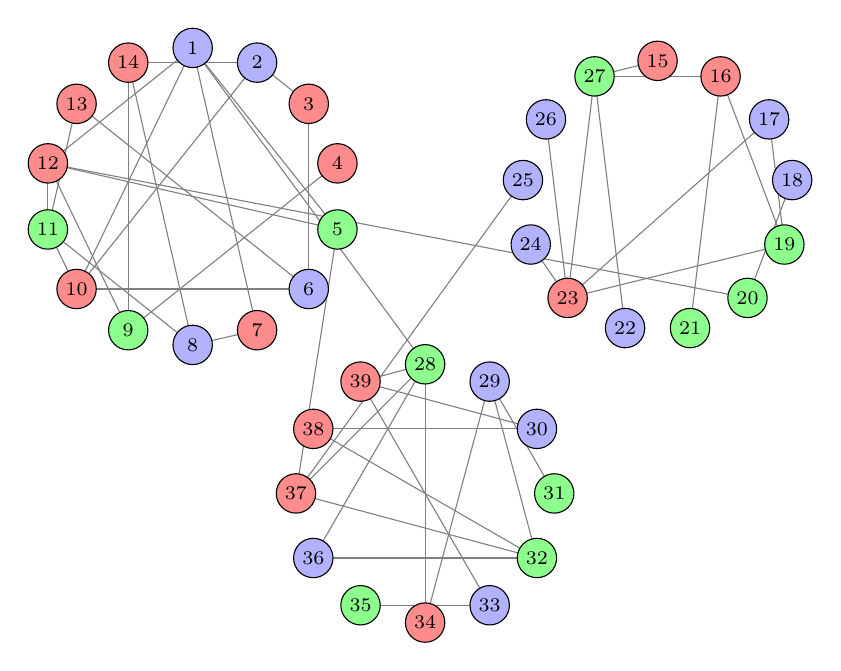
\begin{tikzpicture}[scale=0.82]
% written by figures/colouring_layout.py; do not edit
\draw[gray] (0.0,2.3) -- (2.242,-0.512);
\draw[gray] (0.0,2.3) -- (0.998,-2.072);
\draw[gray] (0.0,2.3) -- (-1.798,-1.434);
\draw[gray] (0.0,2.3) -- (-2.242,0.512);
\draw[gray] (0.0,2.3) -- (3.6,-2.6);
\draw[gray] (0.998,2.072) -- (1.798,1.434);
\draw[gray] (0.998,2.072) -- (-1.798,-1.434);
\draw[gray] (0.998,2.072) -- (-0.998,2.072);
\draw[gray] (1.798,1.434) -- (1.798,-1.434);
\draw[gray] (2.242,0.512) -- (-0.998,-2.072);
\draw[gray] (2.242,-0.512) -- (-2.242,0.512);
\draw[gray] (2.242,-0.512) -- (1.6,-4.6);
\draw[gray] (1.798,-1.434) -- (-1.798,-1.434);
\draw[gray] (1.798,-1.434) -- (-1.798,1.434);
\draw[gray] (0.998,-2.072) -- (0.0,-2.3);
\draw[gray] (0.0,-2.3) -- (-2.242,-0.512);
\draw[gray] (0.0,-2.3) -- (-0.998,2.072);
\draw[gray] (-0.998,-2.072) -- (-2.242,0.512);
\draw[gray] (-0.998,-2.072) -- (-0.998,2.072);
\draw[gray] (-1.798,-1.434) -- (-2.242,-0.512);
\draw[gray] (-2.242,-0.512) -- (-2.242,0.512);
\draw[gray] (-2.242,-0.512) -- (-1.798,1.434);
\draw[gray] (-2.242,0.512) -- (8.593,-1.572);
\draw[gray] (7.2,2.1) -- (6.224,1.859);
\draw[gray] (8.176,1.859) -- (9.164,-0.745);
\draw[gray] (8.176,1.859) -- (7.703,-2.039);
\draw[gray] (8.176,1.859) -- (6.224,1.859);
\draw[gray] (8.928,1.193) -- (9.164,-0.745);
\draw[gray] (8.928,1.193) -- (5.807,-1.572);
\draw[gray] (9.285,0.253) -- (8.593,-1.572);
\draw[gray] (9.164,-0.745) -- (5.807,-1.572);
\draw[gray] (6.697,-2.039) -- (6.224,1.859);
\draw[gray] (5.807,-1.572) -- (5.236,-0.745);
\draw[gray] (5.807,-1.572) -- (5.472,1.193);
\draw[gray] (5.807,-1.572) -- (6.224,1.859);
\draw[gray] (5.115,0.253) -- (1.6,-4.6);
\draw[gray] (3.6,-2.6) -- (3.6,-6.6);
\draw[gray] (3.6,-2.6) -- (1.868,-5.6);
\draw[gray] (3.6,-2.6) -- (1.6,-4.6);
\draw[gray] (3.6,-2.6) -- (2.6,-2.868);
\draw[gray] (4.6,-2.868) -- (5.6,-4.6);
\draw[gray] (4.6,-2.868) -- (5.332,-5.6);
\draw[gray] (4.6,-2.868) -- (3.6,-6.6);
\draw[gray] (5.332,-3.6) -- (1.868,-3.6);
\draw[gray] (5.332,-3.6) -- (2.6,-2.868);
\draw[gray] (5.332,-5.6) -- (1.868,-5.6);
\draw[gray] (5.332,-5.6) -- (1.6,-4.6);
\draw[gray] (5.332,-5.6) -- (1.868,-3.6);
\draw[gray] (4.6,-6.332) -- (2.6,-6.332);
\draw[gray] (4.6,-6.332) -- (2.6,-2.868);
\node[circle, draw, minimum size=5mm, inner sep=0pt, font=\scriptsize, fill=blue!30] at (0.0,2.3) {1};
\node[circle, draw, minimum size=5mm, inner sep=0pt, font=\scriptsize, fill=blue!30] at (0.998,2.072) {2};
\node[circle, draw, minimum size=5mm, inner sep=0pt, font=\scriptsize, fill=red!45] at (1.798,1.434) {3};
\node[circle, draw, minimum size=5mm, inner sep=0pt, font=\scriptsize, fill=red!45] at (2.242,0.512) {4};
\node[circle, draw, minimum size=5mm, inner sep=0pt, font=\scriptsize, fill=green!45] at (2.242,-0.512) {5};
\node[circle, draw, minimum size=5mm, inner sep=0pt, font=\scriptsize, fill=blue!30] at (1.798,-1.434) {6};
\node[circle, draw, minimum size=5mm, inner sep=0pt, font=\scriptsize, fill=red!45] at (0.998,-2.072) {7};
\node[circle, draw, minimum size=5mm, inner sep=0pt, font=\scriptsize, fill=blue!30] at (0.0,-2.3) {8};
\node[circle, draw, minimum size=5mm, inner sep=0pt, font=\scriptsize, fill=green!45] at (-0.998,-2.072) {9};
\node[circle, draw, minimum size=5mm, inner sep=0pt, font=\scriptsize, fill=red!45] at (-1.798,-1.434) {10};
\node[circle, draw, minimum size=5mm, inner sep=0pt, font=\scriptsize, fill=green!45] at (-2.242,-0.512) {11};
\node[circle, draw, minimum size=5mm, inner sep=0pt, font=\scriptsize, fill=red!45] at (-2.242,0.512) {12};
\node[circle, draw, minimum size=5mm, inner sep=0pt, font=\scriptsize, fill=red!45] at (-1.798,1.434) {13};
\node[circle, draw, minimum size=5mm, inner sep=0pt, font=\scriptsize, fill=red!45] at (-0.998,2.072) {14};
\node[circle, draw, minimum size=5mm, inner sep=0pt, font=\scriptsize, fill=red!45] at (7.2,2.1) {15};
\node[circle, draw, minimum size=5mm, inner sep=0pt, font=\scriptsize, fill=red!45] at (8.176,1.859) {16};
\node[circle, draw, minimum size=5mm, inner sep=0pt, font=\scriptsize, fill=blue!30] at (8.928,1.193) {17};
\node[circle, draw, minimum size=5mm, inner sep=0pt, font=\scriptsize, fill=blue!30] at (9.285,0.253) {18};
\node[circle, draw, minimum size=5mm, inner sep=0pt, font=\scriptsize, fill=green!45] at (9.164,-0.745) {19};
\node[circle, draw, minimum size=5mm, inner sep=0pt, font=\scriptsize, fill=green!45] at (8.593,-1.572) {20};
\node[circle, draw, minimum size=5mm, inner sep=0pt, font=\scriptsize, fill=green!45] at (7.703,-2.039) {21};
\node[circle, draw, minimum size=5mm, inner sep=0pt, font=\scriptsize, fill=blue!30] at (6.697,-2.039) {22};
\node[circle, draw, minimum size=5mm, inner sep=0pt, font=\scriptsize, fill=red!45] at (5.807,-1.572) {23};
\node[circle, draw, minimum size=5mm, inner sep=0pt, font=\scriptsize, fill=blue!30] at (5.236,-0.745) {24};
\node[circle, draw, minimum size=5mm, inner sep=0pt, font=\scriptsize, fill=blue!30] at (5.115,0.253) {25};
\node[circle, draw, minimum size=5mm, inner sep=0pt, font=\scriptsize, fill=blue!30] at (5.472,1.193) {26};
\node[circle, draw, minimum size=5mm, inner sep=0pt, font=\scriptsize, fill=green!45] at (6.224,1.859) {27};
\node[circle, draw, minimum size=5mm, inner sep=0pt, font=\scriptsize, fill=green!45] at (3.6,-2.6) {28};
\node[circle, draw, minimum size=5mm, inner sep=0pt, font=\scriptsize, fill=blue!30] at (4.6,-2.868) {29};
\node[circle, draw, minimum size=5mm, inner sep=0pt, font=\scriptsize, fill=blue!30] at (5.332,-3.6) {30};
\node[circle, draw, minimum size=5mm, inner sep=0pt, font=\scriptsize, fill=green!45] at (5.6,-4.6) {31};
\node[circle, draw, minimum size=5mm, inner sep=0pt, font=\scriptsize, fill=green!45] at (5.332,-5.6) {32};
\node[circle, draw, minimum size=5mm, inner sep=0pt, font=\scriptsize, fill=blue!30] at (4.6,-6.332) {33};
\node[circle, draw, minimum size=5mm, inner sep=0pt, font=\scriptsize, fill=red!45] at (3.6,-6.6) {34};
\node[circle, draw, minimum size=5mm, inner sep=0pt, font=\scriptsize, fill=green!45] at (2.6,-6.332) {35};
\node[circle, draw, minimum size=5mm, inner sep=0pt, font=\scriptsize, fill=blue!30] at (1.868,-5.6) {36};
\node[circle, draw, minimum size=5mm, inner sep=0pt, font=\scriptsize, fill=red!45] at (1.6,-4.6) {37};
\node[circle, draw, minimum size=5mm, inner sep=0pt, font=\scriptsize, fill=red!45] at (1.868,-3.6) {38};
\node[circle, draw, minimum size=5mm, inner sep=0pt, font=\scriptsize, fill=red!45] at (2.6,-2.868) {39};

\end{tikzpicture}
\par\smallskip{\small The friendship graph coloured by the \omterm{def:b1:propositional-logic:model}{model} of \cref{out:b1:propositional-logic:colouring}: red,
green and blue. No edge joins two vertices of the same colour. Two colours fail because the graph has a cycle of odd
length (the friends 1, 5 and 12 form a triangle), which cannot alternate between two colours.}
\end{omfigure}

The \omterm{def:b1:propositional-logic:literal}{clauses} do not say that a person has at most one colour. They need not: in a \omterm{def:b1:propositional-logic:model}{model} where a person has two, either
colour can be kept, and the program keeps the first. Leaving out \omterm{def:b1:propositional-logic:literal}{clauses} that cannot change the answer keeps the
encoding small; adding them makes the \omterm{def:b1:propositional-logic:model}{model} easier to read. Either way, the \omterm{def:b1:propositional-logic:model}{model} is checked against the \omterm{def:b1:propositional-logic:literal}{clauses} before
it is used, and the \omterm{def:b1:propositional-logic:colouring}{colouring} against the edges.

\begin{safety}
A \omterm{def:b1:propositional-logic:model}{model} is only as good as the encoding. A forgotten rule gives \omterm{def:b1:propositional-logic:model}{models} that obey the formula and not the world; a wrong
rule can make the formula unsatisfiable and the problem seem impossible. Check a \omterm{def:b1:propositional-logic:model}{model} against the original
constraints with a separate program, and test the encoding on cases small enough to enumerate.
\end{safety}

\section{Exercises}\label{sec:b1:propositional-logic:exercises}

\begin{exercise}[$\star$]\label{exo:b1:propositional-logic:1}
Give the \omterm{def:b1:propositional-logic:valuation}{truth value} of $\neg(p \wedge q) \rightarrow (r \vee \neg p)$ when $p$ is true and $q$, $r$ are false.
\end{exercise}

\begin{exercise}[$\star$]\label{exo:b1:propositional-logic:2}
Draw the tree of $((p \vee \neg q) \rightarrow r) \wedge \neg\neg p$. Give its \omterm{def:b1:propositional-logic:size}{size}, its \omterm{def:b1:propositional-logic:size}{height} and the number of its
\omterm{def:b1:propositional-logic:size}{subformulas}.
\end{exercise}

\begin{exercise}[$\star$]\label{exo:b1:propositional-logic:3}
Which of these formulas are tautologies, which are antilogies, and which are neither?
(a) $(p \rightarrow q) \rightarrow (\neg q \rightarrow \neg p)$; (b) $(p \rightarrow q) \rightarrow (q \rightarrow p)$;
(c) $p \vee (p \rightarrow q)$; (d) $\neg(p \rightarrow (q \rightarrow p))$.
\end{exercise}

\begin{exercise}[$\star$]\label{exo:b1:propositional-logic:4}
Predict what the program prints, simplified forms included.
\omcode{code/bachelor-1/10-propositional-logic/listings/exo_nf.py}{6}{11}{Three normal forms}
\end{exercise}

\begin{exercise}[$\star\star$]\label{exo:b1:propositional-logic:5}
A student's evaluator reads $p \rightarrow q$ as ``if $p$ then $q$'', with the table below. Find the error from the
printed rows, explain why \code{p >> p} is no longer a \omterm{def:b1:propositional-logic:model}{tautology}, and correct the table.
\omcode{code/bachelor-1/10-propositional-logic/listings/exo_imp.py}{6}{8}{The implication of the student}
\omoutput[2-4]{code/bachelor-1/10-propositional-logic/outputs/exo_imp.txt}{Rows for (F,F), (F,T), (T,F), (T,T).}
\end{exercise}

\begin{exercise}[$\star\star$]\label{exo:b1:propositional-logic:6}
This converter puts all the \omterm{def:b1:propositional-logic:literal}{literals} of a disjunction in one \omterm{def:b1:propositional-logic:literal}{clause}. Find a formula on which it is wrong, explain the
mistake with distributivity, and say on which formulas it is right.
\omcode{code/bachelor-1/10-propositional-logic/listings/exo_cnf_bug.py}{8}{19}{A converter that does not distribute}
\omoutput[2-4]{code/bachelor-1/10-propositional-logic/outputs/exo_cnf_bug.txt}{Its answer on $p \vee (q \wedge r)$.}
\end{exercise}

\begin{exercise}[$\star\star$]\label{exo:b1:propositional-logic:7}
Write \code{is_consequence(gamma, phi)}, which decides $\Gamma \models \varphi$ by trying every \omterm{def:b1:propositional-logic:valuation}{valuation} of the
variables of $\Gamma$ and $\varphi$. Test it on $\{p, p \rightarrow q\} \models q$, on $\{q, p \rightarrow q\}
\not\models p$, and on $\{p, \neg p\} \models q$; explain the last one.
\end{exercise}

\begin{exercise}[$\star\star$]\label{exo:b1:propositional-logic:8}
Write \code{exactly_one(lits)}, which returns \omterm{def:b1:propositional-logic:literal}{clauses} true exactly when one of the given \omterm{def:b1:propositional-logic:literal}{literals} is true, and test it
by counting the \omterm{def:b1:propositional-logic:model}{models} for up to six \omterm{def:b1:propositional-logic:literal}{literals}.
\end{exercise}

\begin{exercise}[$\star\star$]\label{exo:b1:propositional-logic:9}
Count the \omterm{def:b1:propositional-logic:literal}{clauses} of the encoding of \cref{exo:b1:propositional-logic:8} for $n$ \omterm{def:b1:propositional-logic:literal}{literals}, and their \omterm{def:b1:propositional-logic:literal}{literals}. How many
\omterm{def:b1:propositional-logic:literal}{clauses} say that each of the 7 members of a committee has exactly one of 7 seats and each seat exactly one member?
\end{exercise}

\begin{exercise}[$\star\star\star$]\label{exo:b1:propositional-logic:10}
Prove that every formula is equivalent to a formula that uses only the \omterm{def:b1:propositional-logic:formula}{connectives} $\neg$ and $\wedge$, by induction
on the formula. What is the \omterm{def:b1:propositional-logic:size}{size} of the result, as a function of the \omterm{def:b1:propositional-logic:size}{size} of the original, if the original has no
$\leftrightarrow$? Why does $\leftrightarrow$ cause a problem?
\end{exercise}

\begin{exercise}[$\star\star\star$]\label{exo:b1:propositional-logic:11}
Write \code{quine_units}, Quine's algorithm with \omterm{def:b1:propositional-logic:unit}{unit propagation} before each choice, counting its nodes. Compare its
node counts with those of \code{quine} on the dinner, the \omterm{def:b1:propositional-logic:colouring}{colourings} with two and three colours, and the committee
of the problem, \omterm{def:b1:propositional-logic:model}{satisfiable} and not.
\end{exercise}

\begin{exercise}[$\star\star\star$]\label{exo:b1:propositional-logic:12}
Prove that $\varphi$ is a \omterm{def:b1:propositional-logic:model}{tautology} if and only if $\neg\varphi$ is unsatisfiable, and deduce a way to test a \omterm{def:b1:propositional-logic:model}{tautology}
with Quine's algorithm. Then prove that \omterm{def:b1:propositional-logic:unit}{unit propagation} never turns a \omterm{def:b1:propositional-logic:model}{satisfiable} set of \omterm{def:b1:propositional-logic:literal}{clauses} into an
unsatisfiable one, nor the converse.
\end{exercise}

\section{Problem: Seating the committee}\label{sec:b1:propositional-logic:problem}

\begin{problem}[{Weekend problem --- Seating the committee}]\label{pb:b1:propositional-logic:1}
Seven members of the town's library committee, Alma, Boris, Chloe, Dmitri, Elena, Farid and Greta (initials A to G),
sit in a row of seven seats, numbered 1 to 7. Six rules constrain the seating: Alma sits next to Boris; Chloe does not
sit next to Dmitri; Elena sits at an end; Greta, who chairs, sits in the middle seat; Farid sits next to Greta; Chloe
sits next to Elena. The variable \code{C6} says that Chloe sits in seat 6. The program writes the rules as formulas,
turns them into \omterm{def:b1:propositional-logic:literal}{clauses} by Tseitin's encoding, adds the \omterm{def:b1:propositional-logic:literal}{clauses} of \cref{exo:b1:propositional-logic:8} for the seats,
solves, and checks the answer against all $7! = 5040$ seatings.
\omcode{code/bachelor-1/10-propositional-logic/listings/tseitin.py}{6}{33}{Tseitin's encoding: one variable per
binary \omterm{def:b1:propositional-logic:formula}{connective}}\label{lst:b1:propositional-logic:tseitin}
\omcode{code/bachelor-1/10-propositional-logic/listings/committee.py}{17}{47}{The committee's
\omterm{def:b1:propositional-logic:literal}{clauses}}\label{lst:b1:propositional-logic:committee}
\omoutput{code/bachelor-1/10-propositional-logic/outputs/committee.txt}{\omterm{def:b1:propositional-logic:size}{Sizes}, \omterm{def:b1:propositional-logic:literal}{clause} counts, a seating, the check, and
one rule too many.}\label{out:b1:propositional-logic:committee}

\medskip\noindent\textbf{Part I --- The encoding.}
\begin{enumerate}
\item How many variables describe a seating? How many \omterm{def:b1:propositional-logic:valuation}{valuations} do they have, and how many of them are seatings?
\item Write the rule ``Alma sits next to Boris'' as \code{next_to} builds it, for seats 1, 2 and 7 only.
\item Check that the formula of ``Alma next to Boris'' has \omterm{def:b1:propositional-logic:size}{size} 37: count its variables and its \omterm{def:b1:propositional-logic:formula}{connectives}.
\item Why is ``Chloe not next to Dmitri'' of \omterm{def:b1:propositional-logic:size}{size} 38?
\item How many \omterm{def:b1:propositional-logic:literal}{clauses} do the seat constraints produce, members and seats together?
\item Check the total of 533 \omterm{def:b1:propositional-logic:literal}{clauses}.
\end{enumerate}

\medskip\noindent\textbf{Part II --- Normal forms and their cost.}
\begin{enumerate}[resume]
\item The naive CNF of ``Alma next to Boris'' has 128 \omterm{def:b1:propositional-logic:literal}{clauses}. Explain the number $2^7$ by distributivity.
\item Why does the naive CNF of ``Chloe not next to Dmitri'' have only 12 \omterm{def:b1:propositional-logic:literal}{clauses}? Write two of them.
\item Is the formula of ``Alma next to Boris'' in DNF? Is ``Elena at an end''?
\item With the seat \omterm{def:b1:propositional-logic:literal}{clauses} in force, ``Alma next to Boris'' is equivalent to a formula of fewer \omterm{def:b1:propositional-logic:literal}{clauses}:
$\bigwedge_s (\neg A_s \vee B_{s-1} \vee B_{s+1})$. Explain why, and count its \omterm{def:b1:propositional-logic:literal}{clauses}.
\item By \cref{prop:b1:propositional-logic:blowup}, which kind of rule would make the naive CNF unusable?
\item Why do the seat constraints need no Tseitin variable?
\end{enumerate}

\medskip\noindent\textbf{Part III --- Tseitin's encoding.}
\begin{enumerate}[resume]
\item Check that the three \omterm{def:b1:propositional-logic:literal}{clauses} of the \code{&} gate say $t \leftrightarrow (a \wedge b)$, by a truth table of eight
rows.
\item Why does a negation need no new variable, and why can equal \omterm{def:b1:propositional-logic:size}{subformulas} share one?
\item Show that from any \omterm{def:b1:propositional-logic:model}{model} of $\varphi$ one obtains a \omterm{def:b1:propositional-logic:model}{model} of \code{tseitin(f)}, by giving each new variable the
value of its \omterm{def:b1:propositional-logic:size}{subformula}.
\item Show that any \omterm{def:b1:propositional-logic:model}{model} of \code{tseitin(f)} is a \omterm{def:b1:propositional-logic:model}{model} of $\varphi$ on the variables of $\varphi$.
\item Deduce that $\varphi$ and \code{tseitin(f)} are \omterm{def:b1:propositional-logic:equisat}{equisatisfiable}, though not equivalent.
\item Prove \emph{Tseitin's theorem}: a formula of \omterm{def:b1:propositional-logic:size}{size} $m$ has an \omterm{def:b1:propositional-logic:equisat}{equisatisfiable} CNF of at most $2m - 1$ \omterm{def:b1:propositional-logic:literal}{clauses}
(hence at most $3m$), each of at most three \omterm{def:b1:propositional-logic:literal}{literals}. Check the bound on the six rules.
\end{enumerate}

\medskip\noindent\textbf{Part IV --- Solving and reading back.}
\begin{enumerate}[resume]
\item Read the seating from the output and check each rule on it.
\item Why do the eight seatings come in pairs? What does each pair have in common?
\item Plain Quine's algorithm took 3219 nodes. In \cref{exo:b1:propositional-logic:11}, with \omterm{def:b1:propositional-logic:unit}{unit propagation}, it
takes 2. Which \omterm{def:b1:propositional-logic:unit}{unit clause} starts the propagation?
\item Show by hand, without any search, that adding ``Farid sits next to Elena'' makes the rules unsatisfiable.
\item Why did the plain algorithm need 182667 nodes to reach the same conclusion?
\item State the named result of the problem, \emph{Tseitin's theorem}, and the committee's count.
\end{enumerate}
\end{problem}
